%##################################################################################################

The tasks within the \texttt{Tool} category of our benchmark are designed to deeply investigate an AI agent's capabilities in tool utilization, precision in tool handling, and contextual application of various tools to carry out specific tasks. This category provides insights into the agent's skill in wielding, using, and exploiting tools optimally within different Minecraft scenarios. 

\begin{figure*}[h]
%\framebox[4.0in]{$\;$}
\begin{center}
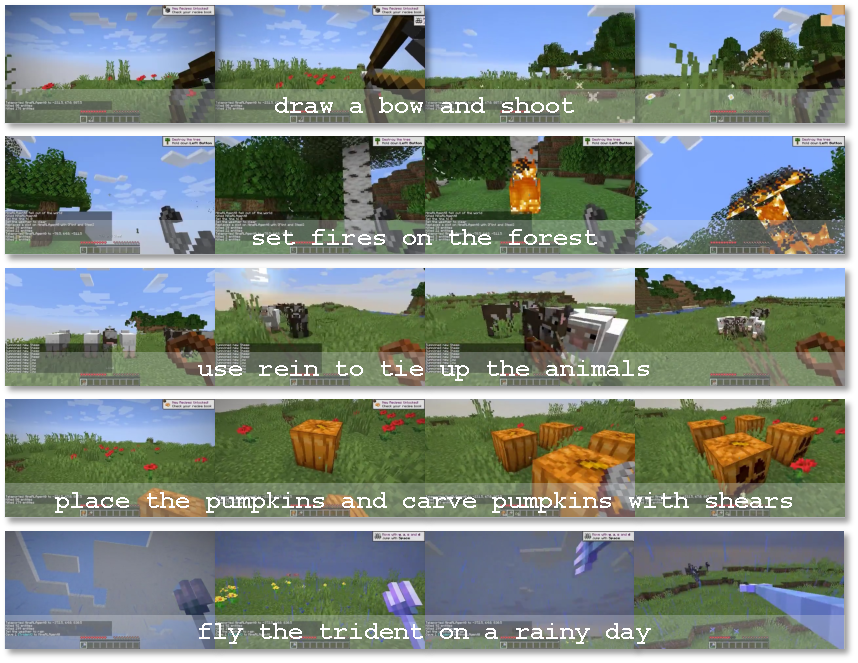
\includegraphics[scale = 0.9]{figures/benchmark_tool.pdf}
\end{center}
\caption{Examples of tasks in \texttt{tool} category. }
\end{figure*}

\definecolor{codeblue}{rgb}{0.25,0.5,0.5}
\definecolor{codekw}{rgb}{0.85, 0.18, 0.50}
\definecolor{keywordgreen}{rgb}{0,0.6,0}
\lstset{
  backgroundcolor=\color{gray!10},
  basicstyle=\fontsize{8pt}{9pt}\ttfamily\selectfont,
  columns=fullflexible,
  breaklines=true,
  captionpos=b,
  commentstyle=\fontsize{7.5pt}{7.5pt}\color{codeblue},
  keywords = {Task, Description, Time, Evaluation, Precondition,SkillAssessed}, 
  keywordstyle = {\textbf},
  caption={The environment configuration and evaluation metric for \texttt{tool} series tasks. },
  label={lst:minecraft_deps_prompt}
}
\begin{lstlisting} % [language=python]  

Task: use bow
Description: Draw a bow and shoot. 
Precondition: Spawn the player in the plains biome with a bow in the mainhand and a stack of arrows in the inventory. 
SkillAssessed: Precision, tool handling, and projectile mastery.
Evaluation: Just run. < Draw the bow and shoot the arrow. < Hold the bow steady and charge up the shot before releasing the arrow.  

Task: set fires
Description: Set fires on the trees. 
Precondition: Spawn the player in the forest biome with a flint_and_steel in its main hand. 
SkillAssessed: Environment manipulation and controlled chaos creation.
Evaluation: Attack the tree. < Start a fire with the flint_and_steel. < Go wild with the fire. 

Task: lead animals
Description: Use rein to tie up the animals. 
Precondition: Spawn the player in the plains biome with a stack of leads in its main hand. Spawn 5 sheep and 5 cows near the player's position. 
SkillAssessed: Entity interaction, tool application on moving entities, and livestock 
Evaluation: Ignore the animals and run away. < Use the rein to tie up animals. 

Task: carve pumpkins
Description: Place the pumpkins and carve pumpkins with shears.
Precondition: Spawn the player in the plains biome with a shear in its main hand and a stack of pumpkins in the inventory. 
SkillAssessed: Block placement, block modification, and crafting interaction.
Evaluation: Just run. < Place the pumpkin on the surface. < Use the shear to carve it. < Get a carved pumpkin. 

Task: use trident
Description: Fly the trident on a rainy day. 
Precondition: Spawn the player in the plains biome with a trident in the main hand, which is enchanted with riptide. The weather is rain. 
SkillAssessed: Weather-adaptive tool utilization, motion dynamics, and advanced weapon handling.
Evaluation: Just run. < Use the trident to break the block. < Use the trident for quick movement. < Charge to throw the trident farther. 

\end{lstlisting}


